\documentclass[a4paper,12pt]{article} % The document class with options

\usepackage[margin=1in]{geometry}
\usepackage{newtxtext,newtxmath}
\usepackage[T1]{fontenc}
\usepackage{amsmath}
\usepackage{amsfonts}
\usepackage{microtype}
\usepackage{graphicx}
% chktex-file 3
% chktex-file 36
% chktex-file 44

\begin{document}
\setlength{\parskip}{1em} 
\setlength{\parindent}{0pt}
\newcommand{\vect}[1]{\mathbf{#1}}

\title{CHBE 552 Problem Set 4}
\author{Jincong Li \\ 60539939}
\date{\today}
\maketitle

\begin{align*}
    \intertext{For Question 1}
    \vect{k} &= [kH, kR , KA]^T \\
    \vect{x} &= [pA]\\
    \intertext{Note this input vector contains information for two different temperatures and will be
    treated separately in the code.}
    \vect{f}_{model A} &= R - \sqrt{R^2 - kH^2} \\
    \text{with} 
    R &= kH + \frac{kH^2}{2kR}\frac{(1+KAp_A)^2}{KAp_A} \\
    \vect{f}_{model B} &= (kH^{\lambda}+(\frac{kRKAp_A}{(1+KAp_A)^2})^2)^{\frac{1}{\lambda}} \\
    \vect{y} &= [rA]\\
    \intertext{The same separate treatment will also be applied to the output vector.}\\
    \intertext{For Question 2}\\
    \vect{k} &= [ko, kp]^T \\
    \vect{x} &= [Cp, Co, n]^T \\
    \vect{f} &= \frac{ko kp {Co}^{0.5} Cp}{ko {Co}^{0.5} + n kp Cp} \\
    \vect{y} &= [rp]
\end{align*} 
The sensitivity matrix of those vector valued functions are equivalent to their Jacobian matrix which
is computed and embeded in the code. Thus, it could not be presented here explicitly, but I shall provide
the computation procedure here:

For a parameter vector $\boldsymbol{\theta}$ of length $n$, and $m$ residuals, the Jacobian matrix $\mathbf{J}$ is an $m \times n$ matrix. The approximation of the $j$-th column of $\mathbf{J}$ (the derivative of the residuals with respect to the $j$-th parameter) can be calculated as follows:

\begin{enumerate}
    \item \textbf{Slightly Perturb the $j$-th Parameter}: For a small value $\varepsilon$, create a new parameter vector $\boldsymbol{\theta}_\varepsilon$ where only the $j$-th parameter is increased by $\varepsilon$, i.e., 
    \[ \theta_{\varepsilon,j} = \theta_j + \varepsilon. \]
    
    \item \textbf{Calculate the Difference in Predictions}: Use the model function to calculate predictions using $\boldsymbol{\theta}$ and $\boldsymbol{\theta}_\varepsilon$, and compute the difference in the resulting predictions. This difference approximates the change in the residuals caused by the perturbation in the $j$-th parameter.
    
    \item \textbf{Divide by $\varepsilon$}: The approximation of the derivative is the difference in the residuals divided by $\varepsilon$.
\end{enumerate}


From now on, result tables for each model and equestions are presented. In table 1, the final results for
those parameters with their corresponding 95\% confidence intervals in each case are listed.

\begin{table}[ht]
    \caption{GN-M Method Results}
    \centering
    \begin{tabular}{|c|c|c|c|}
        \hline
        Q1 & kH \& CI & kR \& CI& KA \& CI\\
        \hline   
        Model A 600& 0.094 [0.069 0.118]& 0.607 [0.400 0.812]& 0.517 [0.390 0.642] \\
        Model A 575& 0.832 [0.779 0.934]& 0.119 [0.112 0.124]& 0.397 [0.352 0.442] \\
        Model B 600& 0.084 [0.064 0.103]& 0.732 [0.515 0.948]& 0.516 [0.346 0.451] \\
        Model B 575& 0.922 [0.834 1.012]& 0.126 [0.118 0.133]& 0.399 [0.352 0.442]\\
        \hline
        Q2 & ko \& CI& kp \& CI&\\
        \hline
        & 1330.8 [1209.5 1407.7] & 0.612 [0.411 0.803] &  \\
        \hline
    \end{tabular}
\end{table}

Note that "CI" refers to 95\% confidence interval.
\begin{table}[ht]
\caption{Results for Model A at T = 600 degree Parameter Estimation of Q1 using modified G-N method}
\centering
\begin{tabular}{|c|c|c|c|c|}
    \hline
    Iteration Number & Objective Function Value & kH & kR & KA \\
    \hline
    1 & 0.000260 & 0.085 & 0.683 & 0.520 \\
2 & 0.000066 & 0.088 & 0.668 & 0.522 \\
3 & 0.000064 & 0.089 & 0.656 & 0.522 \\
4 & 0.000064 & 0.090 & 0.646 & 0.521 \\
5 & 0.000064 & 0.091 & 0.638 & 0.520 \\
6 & 0.000064 & 0.092 & 0.631 & 0.519 \\
7 & 0.000063 & 0.092 & 0.626 & 0.519 \\
8 & 0.000063 & 0.092 & 0.621 & 0.518 \\
9 & 0.000063 & 0.093 & 0.618 & 0.518 \\
10 & 0.000063 & 0.093 & 0.616 & 0.518 \\
11 & 0.000063 & 0.093 & 0.613 & 0.517 \\
12 & 0.000063 & 0.093 & 0.612 & 0.517 \\
13 & 0.000063 & 0.094 & 0.611 & 0.517 \\
14 & 0.000063 & 0.094 & 0.610 & 0.517 \\
15 & 0.000063 & 0.094 & 0.609 & 0.517 \\
16 & 0.000063 & 0.094 & 0.608 & 0.517 \\
17 & 0.000063 & 0.094 & 0.608 & 0.517 \\
18 & 0.000063 & 0.094 & 0.608 & 0.517 \\
19 & 0.000063 & 0.094 & 0.607 & 0.517 \\
20 & 0.000063 & 0.094 & 0.607 & 0.517 \\
21 & 0.000063 & 0.094 & 0.607 & 0.517 \\
22 & 0.000063 & 0.094 & 0.607 & 0.517 \\
23 & 0.000063 & 0.094 & 0.607 & 0.517 \\
    \hline
\end{tabular}
\end{table}


\begin{table}[ht]
    \caption{Results for Model A at T = 575 degree Parameter Estimation of Q1 using modified G-N method}
    \centering
    \begin{tabular}{|c|c|c|c|c|}
        \hline
        Iteration Number & Objective Function Value & kH & kR & KA \\
        \hline
        1 & 0.000889 & 0.109 & 0.177 & 0.472 \\
2 & 0.000013 & 0.127 & 0.172 & 0.447 \\
3 & 0.000006 & 0.142 & 0.163 & 0.431 \\
4 & 0.000005 & 0.157 & 0.157 & 0.421 \\
5 & 0.000004 & 0.171 & 0.152 & 0.415 \\
6 & 0.000003 & 0.183 & 0.149 & 0.412 \\
7 & 0.000003 & 0.194 & 0.146 & 0.410 \\
8 & 0.000003 & 0.203 & 0.145 & 0.408 \\
9 & 0.000003 & 0.212 & 0.143 & 0.407 \\
10 & 0.000003 & 0.219 & 0.142 & 0.407 \\
11 & 0.000002 & 0.226 & 0.141 & 0.406 \\
12 & 0.000002 & 0.233 & 0.140 & 0.406 \\
13 & 0.000002 & 0.239 & 0.139 & 0.405 \\
14 & 0.000002 & 0.245 & 0.138 & 0.405 \\
15 & 0.000002 & 0.250 & 0.137 & 0.405 \\
16 & 0.000002 & 0.256 & 0.137 & 0.405 \\
17 & 0.000002 & 0.260 & 0.136 & 0.404 \\
18 & 0.000002 & 0.265 & 0.136 & 0.404 \\
19 & 0.000002 & 0.270 & 0.135 & 0.404 \\
20 & 0.000002 & 0.274 & 0.135 & 0.404 \\
21 & 0.000002 & 0.278 & 0.135 & 0.404 \\
22 & 0.000002 & 0.282 & 0.134 & 0.403 \\
23 & 0.000002 & 0.286 & 0.134 & 0.403 \\
24 & 0.000002 & 0.290 & 0.134 & 0.403 \\
25 & 0.000002 & 0.293 & 0.133 & 0.403 \\
26 & 0.000002 & 0.297 & 0.133 & 0.403 \\
27 & 0.000002 & 0.300 & 0.133 & 0.403 \\
28 & 0.000002 & 0.303 & 0.132 & 0.403 \\
29 & 0.000002 & 0.306 & 0.132 & 0.403 \\
30 & 0.000002 & 0.310 & 0.132 & 0.403 \\
\ldots & \ldots & \ldots & \ldots & \ldots \\
996 & 0.000001 & 0.831 & 0.119 & 0.397 \\
997 & 0.000001 & 0.831 & 0.119 & 0.397 \\
998 & 0.000001 & 0.832 & 0.119 & 0.397 \\
999 & 0.000001 & 0.832 & 0.119 & 0.397 \\
1000 & 0.000001 & 0.832 & 0.119 & 0.397 \\

        \hline
\end{tabular}
\end{table}
    
\begin{table}[ht]
    \caption{Results for Model B at T = 600 degree Parameter Estimation of Q1 using modified G-N method}
    \centering
    \begin{tabular}{|c|c|c|c|c|}
        \hline
        Iteration Number & Objective Function Value & kH & kR & KA \\
        \hline   
        1 & 0.000092 & 0.094 & 0.628 & 0.504 \\
        2 & 0.000066 & 0.091 & 0.649 & 0.506 \\
        3 & 0.000065 & 0.090 & 0.665 & 0.508 \\
        4 & 0.000064 & 0.088 & 0.678 & 0.510 \\
        5 & 0.000064 & 0.087 & 0.688 & 0.511 \\
        6 & 0.000064 & 0.087 & 0.696 & 0.512 \\
        7 & 0.000064 & 0.086 & 0.702 & 0.512 \\
        8 & 0.000064 & 0.086 & 0.707 & 0.513 \\
        9 & 0.000064 & 0.085 & 0.712 & 0.513 \\
        10 & 0.000064 & 0.085 & 0.715 & 0.514 \\
        11 & 0.000064 & 0.085 & 0.718 & 0.514 \\
        12 & 0.000064 & 0.085 & 0.721 & 0.514 \\
        13 & 0.000063 & 0.084 & 0.723 & 0.515 \\
        14 & 0.000063 & 0.084 & 0.724 & 0.515 \\
        15 & 0.000063 & 0.084 & 0.726 & 0.515 \\
        16 & 0.000063 & 0.084 & 0.727 & 0.515 \\
        17 & 0.000063 & 0.084 & 0.728 & 0.515 \\
        18 & 0.000063 & 0.084 & 0.728 & 0.515 \\
        19 & 0.000063 & 0.084 & 0.729 & 0.515 \\
        20 & 0.000063 & 0.084 & 0.730 & 0.515 \\
        21 & 0.000063 & 0.084 & 0.730 & 0.515 \\
        22 & 0.000063 & 0.084 & 0.731 & 0.515 \\
        23 & 0.000063 & 0.084 & 0.731 & 0.515 \\
        24 & 0.000063 & 0.084 & 0.731 & 0.515 \\
        25 & 0.000063 & 0.084 & 0.731 & 0.515 \\
        26 & 0.000063 & 0.084 & 0.732 & 0.515 \\
        27 & 0.000063 & 0.084 & 0.732 & 0.516 \\
        28 & 0.000063 & 0.084 & 0.732 & 0.516 \\
        29 & 0.000063 & 0.084 & 0.732 & 0.516 \\
        30 & 0.000063 & 0.084 & 0.732 & 0.516 \\
        \hline
    \end{tabular}
    \end{table}
    
    \begin{table}[ht]
        \caption{Results for Model B at T = 575 degree Parameter Estimation of Q1 using modified G-N method}
        \centering
        \begin{tabular}{|c|c|c|c|c|}
            \hline
            Iteration Number & Objective Function Value & kH & kR & KA \\
            \hline   
            1 & 0.001072 & 0.033 & 0.564 & 0.512 \\
            2 & 0.000095 & 0.042 & 0.555 & 0.515 \\
            3 & 0.000021 & 0.043 & 0.542 & 0.517 \\
            4 & 0.000020 & 0.044 & 0.529 & 0.518 \\
            5 & 0.000019 & 0.045 & 0.516 & 0.518 \\
            6 & 0.000019 & 0.045 & 0.502 & 0.517 \\
            7 & 0.000019 & 0.046 & 0.489 & 0.515 \\
            8 & 0.000018 & 0.047 & 0.475 & 0.513 \\
            9 & 0.000018 & 0.048 & 0.460 & 0.511 \\
            10 & 0.000018 & 0.049 & 0.445 & 0.507 \\
            11 & 0.000017 & 0.050 & 0.430 & 0.504 \\
            12 & 0.000017 & 0.051 & 0.414 & 0.500 \\
            13 & 0.000016 & 0.052 & 0.397 & 0.495 \\
            14 & 0.000016 & 0.054 & 0.380 & 0.490 \\
            15 & 0.000015 & 0.056 & 0.361 & 0.485 \\
            16 & 0.000014 & 0.059 & 0.342 & 0.479 \\
            17 & 0.000014 & 0.062 & 0.322 & 0.472 \\
            18 & 0.000013 & 0.066 & 0.300 & 0.466 \\
            19 & 0.000012 & 0.071 & 0.278 & 0.458 \\
            20 & 0.000011 & 0.079 & 0.255 & 0.450 \\
            21 & 0.000009 & 0.089 & 0.232 & 0.442 \\
            22 & 0.000008 & 0.103 & 0.212 & 0.434 \\
            23 & 0.000007 & 0.120 & 0.195 & 0.427 \\
            24 & 0.000006 & 0.137 & 0.184 & 0.421 \\
            25 & 0.000005 & 0.153 & 0.177 & 0.417 \\
            26 & 0.000004 & 0.166 & 0.172 & 0.414 \\
            27 & 0.000004 & 0.178 & 0.168 & 0.412 \\
            28 & 0.000003 & 0.189 & 0.165 & 0.411 \\
            29 & 0.000003 & 0.199 & 0.163 & 0.410 \\
            30 & 0.000003 & 0.207 & 0.161 & 0.409 \\
            \ldots & \ldots & \ldots & \ldots & \ldots \\
            996 & 0.000001 & 0.922 & 0.126 & 0.399 \\
997 & 0.000001 & 0.923 & 0.126 & 0.399 \\
998 & 0.000001 & 0.923 & 0.126 & 0.399 \\
999 & 0.000001 & 0.923 & 0.126 & 0.399 \\
1000 & 0.000001 & 0.923 & 0.126 & 0.399 \\
\hline
\end{tabular}
\end{table}

\clearpage
We can see here, that for the situation of 600 degrees, those three parameters converge but not for the 575 degrees situation.
The reason for that might be the lack of data points in the later case. For converged cases, the values of the parameters
generally agree with the values shown on the reference but some error appears. The reason for those errors is unclear up to this 
stage. I tried tuning the modified GN method with various ranges of involved parameters but still could not get closer to the reference
value. There might be some limitations in the code since I implemented the code in a straightforward and efficient way which might lead to 
uncertainties. I also compared the estimated data from the determined parameters with the experimental data and the results for each case
are presented below from figure 1 to 3. We can see here the models for question 1 with estimated parameters actually predict the output well enough with
some error, whereas the values of those parameters seem a little bit further from the reference values. Nevertheless, the situation
looks different for question 2, though the comparison between the estimated data and experimental data looks quite off, the values
of estimated parameters are very close to the reference values. The reason is still unclear and requires further investigation in future.
Regarding the uncertainties related to those parameters, one can conclude that their 95\% confidence intervals are good enough. In fact, almost all the 
reference values for those parameters stay in the estimated 95\% confidence intervals, which verifies the implemented method to some extent.
% \clearpage
\begin{figure}[ht]
    \centering
    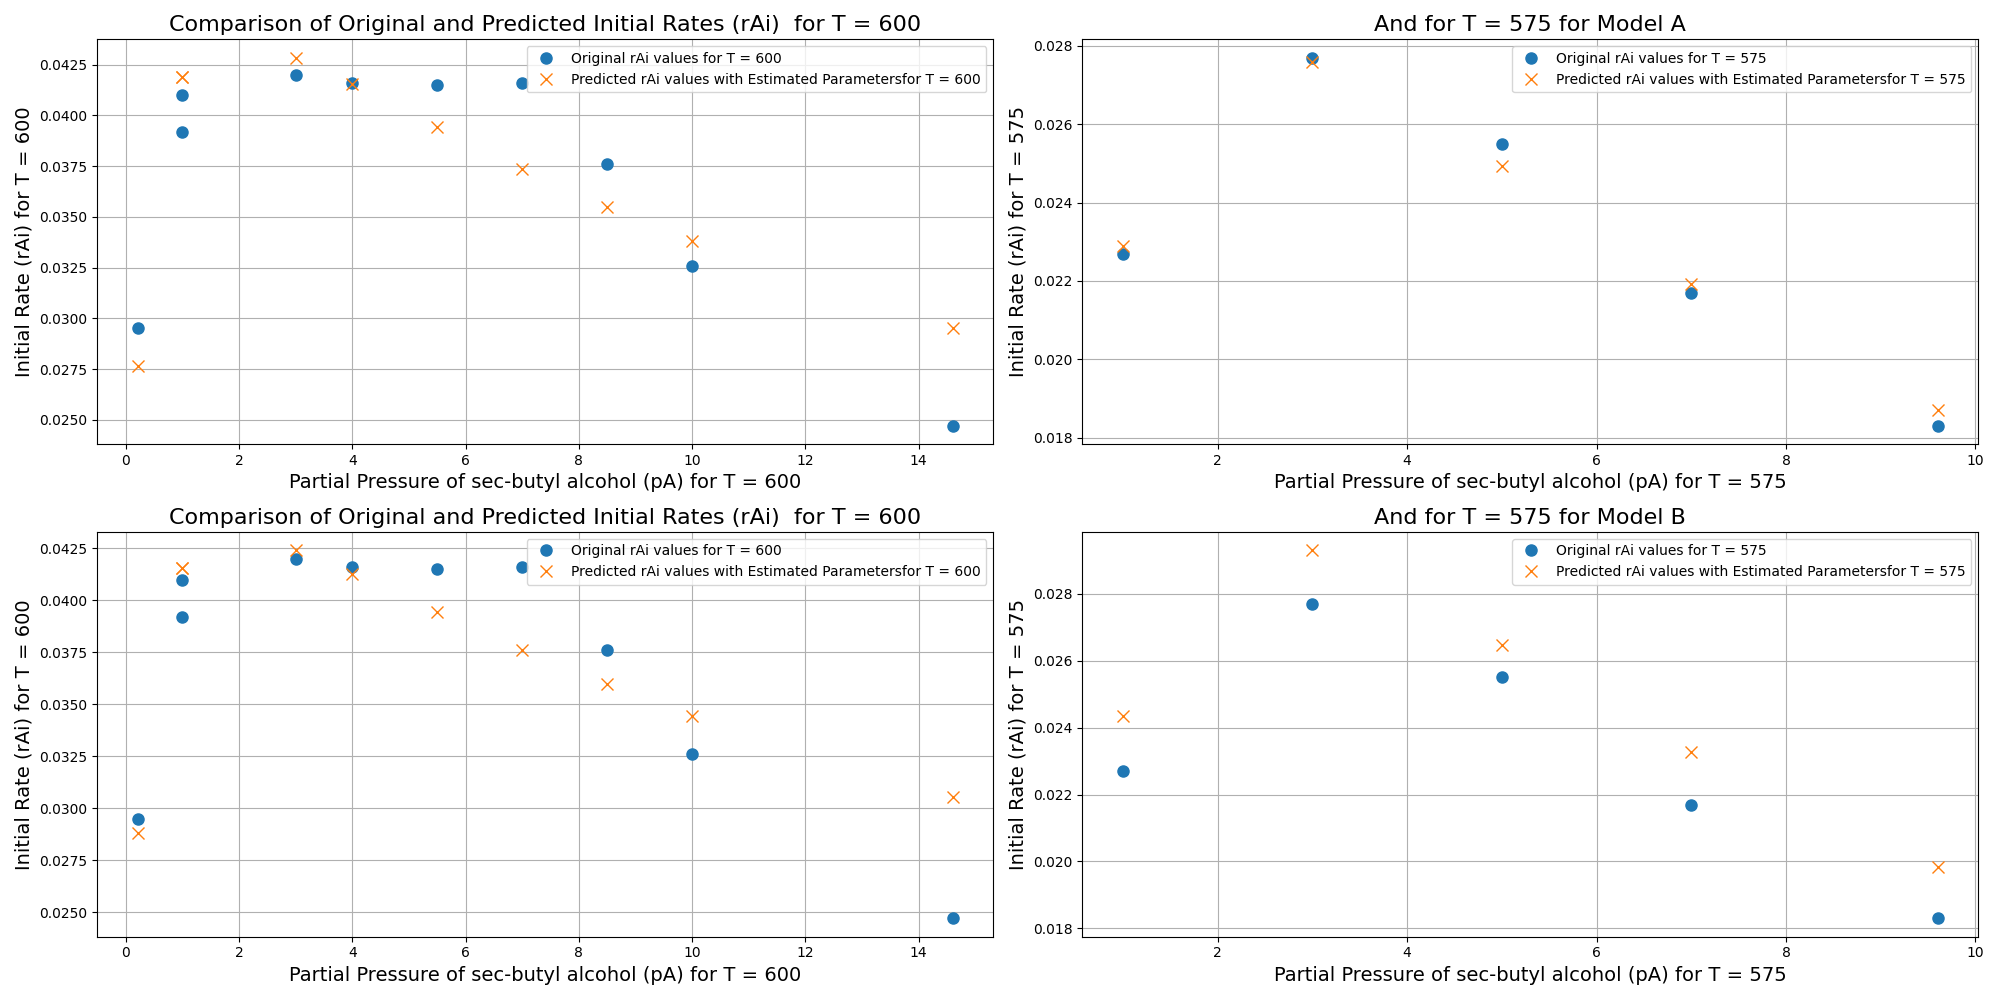
\includegraphics[width=1\textwidth]{GNM_Q1_ParamComp.png}
    \caption{GNM Q1 Data Comparison}
\end{figure}

\begin{figure}[ht]
    \centering
    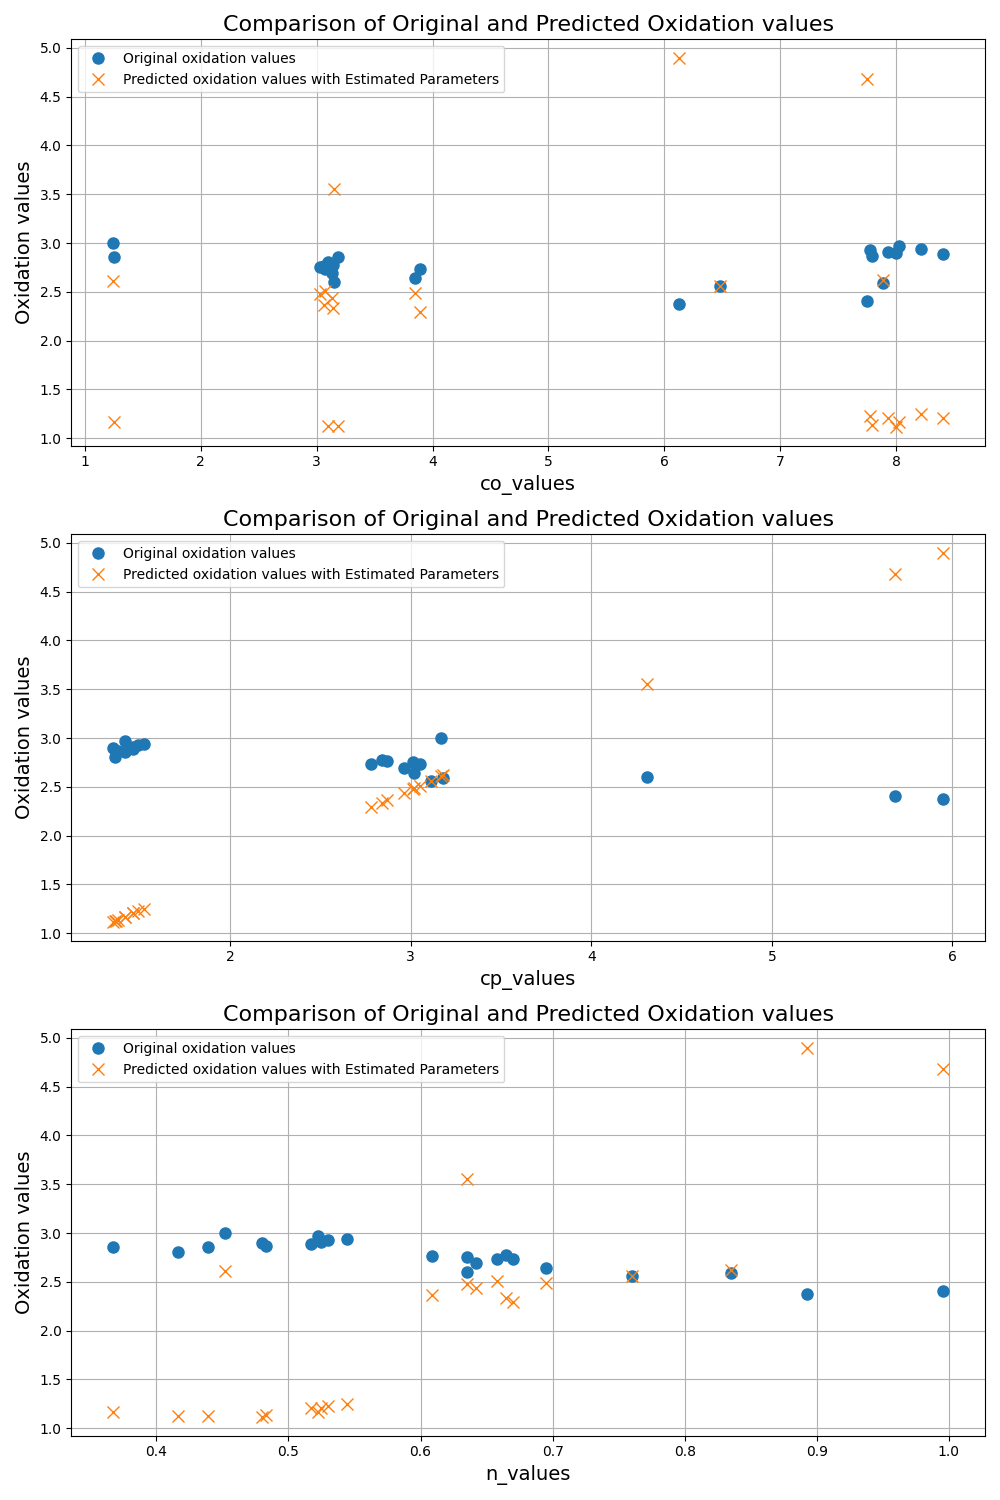
\includegraphics[width=1\textwidth]{GNM_Q2_ParamComp.png}
    \caption{GNM Q2 Data Comparison }
\end{figure}

\begin{figure}[ht]
    \centering
    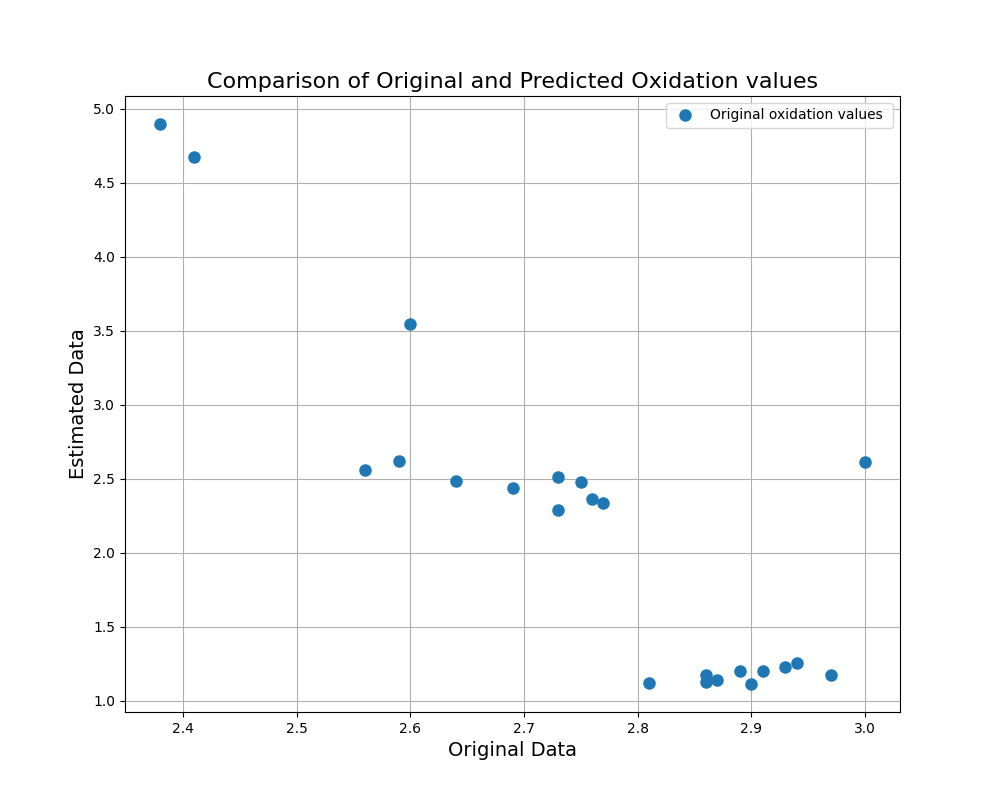
\includegraphics[width=1\textwidth]{GNM_Q2_ParamComp_1.png}
    \caption{GNM Q2 Estimated Data vs. Original Data}
\end{figure}

\clearpage

In table 6, the results of those parameters estimated by the Luus-Jaakola Method are presented. As we can see, they are all 
quite different than the reference values. Since the Luus-Jaakola Method is actually a random process of seeking global 
minimum, the result highly relies on the initial condition/guess of the parameters as well as the number of iterations, 
given in limited performance/executing time of the code, in this case, the Luus-Jaakola Method did not reach the real 
solution that we are looking for. By the experience with tuning parameters in the last assignment, one could definitely
make the LJ method converge to the real solution but it requires too much effort and the time limitation does not allow it. 
Thus, with further work, the LJ method could also return useful information.
\begin{table}[ht]
    \caption{LJ Method Results}
    \centering
    \begin{tabular}{|c|c|c|c|}
        \hline
        Q1 & kH & kR & KA \\
        \hline   
        Model A 600& 0.0876& 0.6444& 0.4261 \\
        Model A 575& 0.1259& 0.0773& 0.3467 \\
        Model B 600& 0.1896& 0.2715& 0.5857 \\
        Model B 575& 0.1610& 0.9212& 0.0468 \\
        \hline
        Q2 & ko & kp&\\
        \hline
         & 1325 & 0.692 &  \\
        \hline
    \end{tabular}
\end{table}



\end{document}